% Capítulo 9: árvore de chamadas de fib(5), com os cálculos repetidos destacados.
\documentclass[border=4pt]{standalone}
\usepackage[utf8]{inputenc}
\usepackage[T1]{fontenc}
% Estilo comum dos fluxogramas e diagramas de blocos.
\usepackage{tikz}
\usetikzlibrary{arrows.meta, positioning, calc, shapes.geometric, shapes.misc}
\definecolor{navy}{RGB}{23,45,80}
\definecolor{laranja}{RGB}{250,110,29}
\definecolor{cinzalogo}{RGB}{107,114,126}
\definecolor{azul}{RGB}{205,222,247}
\tikzset{
  base/.style={draw=navy, line width=0.9pt, font=\sffamily\small, align=center, inner sep=4pt},
  terminal/.style={base, rounded rectangle, fill=laranja!45, draw=laranja, minimum width=20mm, minimum height=7mm},
  processo/.style={base, rectangle, fill=laranja!12, minimum width=28mm, minimum height=8mm},
  decisao/.style={base, diamond, aspect=2.2, fill=azul, inner sep=1pt, minimum width=30mm},
  es/.style={base, trapezium, trapezium left angle=72, trapezium right angle=108,
             fill=white, minimum width=26mm, minimum height=8mm, trapezium stretches body},
  fluxo/.style={-{Stealth[length=2.2mm]}, navy, line width=0.9pt},
  rotulo/.style={font=\sffamily\small\bfseries, text=navy},
  legenda/.style={font=\sffamily\scriptsize, text=cinzalogo},
  resposta/.style={font=\sffamily\scriptsize\bfseries, text=navy},
}

\tikzset{
  f/.style={draw=navy, line width=0.8pt, rounded corners=2pt, fill=white, font=\ttfamily\scriptsize, inner sep=2.5pt},
  f3/.style={f, fill=azul},
  f2/.style={f, fill=laranja!40, draw=laranja},
  edge from parent/.style={draw=navy, line width=0.6pt},
}
\begin{document}
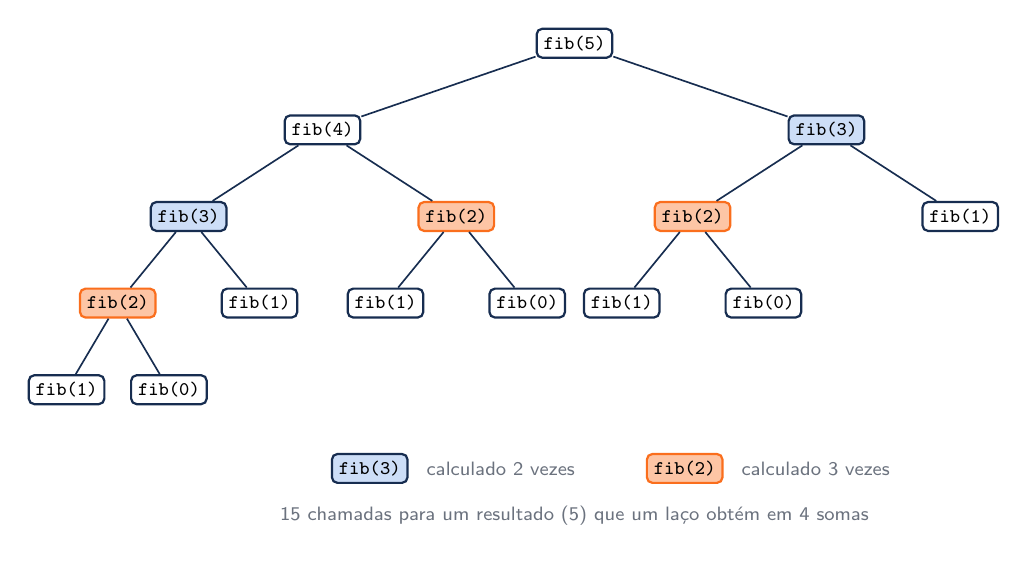
\begin{tikzpicture}[
  level distance=11mm,
  level 1/.style={sibling distance=64mm},
  level 2/.style={sibling distance=34mm},
  level 3/.style={sibling distance=18mm},
  level 4/.style={sibling distance=13mm},
]
  \node[f] {fib(5)}
    child { node[f] {fib(4)}
      child { node[f3] {fib(3)}
        child { node[f2] {fib(2)}
          child { node[f] {fib(1)} }
          child { node[f] {fib(0)} } }
        child { node[f] {fib(1)} } }
      child { node[f2] {fib(2)}
        child { node[f] {fib(1)} }
        child { node[f] {fib(0)} } } }
    child { node[f3] {fib(3)}
      child { node[f2] {fib(2)}
        child { node[f] {fib(1)} }
        child { node[f] {fib(0)} } }
      child { node[f] {fib(1)} } };
  \node[f3] at (-2.6, -5.4) {fib(3)};
  \node[legenda, anchor=west] at (-2.0, -5.4) {calculado 2 vezes};
  \node[f2] at (1.4, -5.4) {fib(2)};
  \node[legenda, anchor=west] at (2.0, -5.4) {calculado 3 vezes};
  \node[legenda] at (0, -6.0) {15 chamadas para um resultado (5) que um laço obtém em 4 somas};
\end{tikzpicture}
\end{document}
